\documentclass{article}
\usepackage{hyperref}
\usepackage{amsmath}
\usepackage{pgfplots}
\usepackage{pgfplotstable}
\pgfplotsset{compat = 1.17}
\pgfplotstableread[col sep=comma]{../results.csv}\results
\title{COMP5329 Assignment 1}
\author{John Hu (zehu4485, 500395897) \and Nicholas Grasevski (ngra5777, 500710654)}
\begin{document}
\maketitle
\begin{abstract}
\end{abstract}

\section{Introduction}
\subsection{Aim}
\subsection{Background}

\section{Methods}
\subsection{Preprocessing}
\subsection{Modules}
\subsubsection{Hidden layer}
\subsubsection{Rectified Linear Unit (ReLU)}
\subsubsection{Weight decay}
\subsubsection{Momentum in Stochastic Gradient Descent (SGD)}
\subsubsection{Dropout}
\subsubsection{Softmax and cross entropy}
\subsubsection{Mini batch training}
\subsubsection{Batch normalization}
\subsection{Design of best model}
\begin{figure}
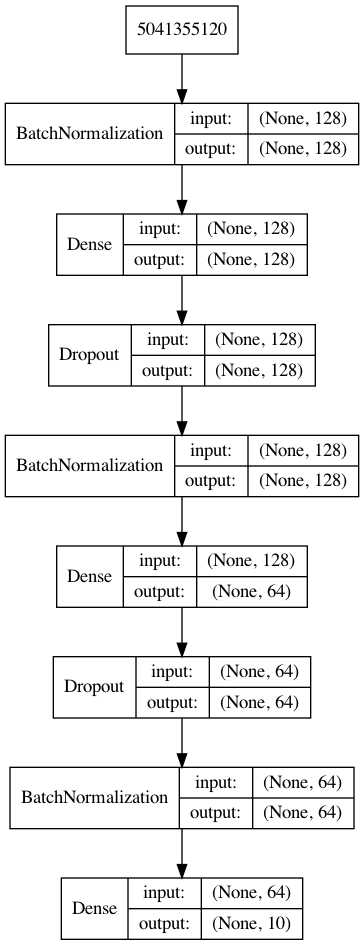
\includegraphics[width=0.5\linewidth]{../model}
\caption{Our best model architecture \label{fig:model}}
\end{figure}

\section{Experiments}
\subsection{Performance}
\subsection{Analysis}
\subsubsection{Hyperparameters}
\subsubsection{Ablation studies}
\subsubsection{Comparison methods}

\section{Results}
\begin{table}\pgfplotstabletypeset[
    every head row/.style={after row=\hline},
]{\results}\caption{
  Train and test log loss mean and standard deviation on different hyperparameter settings.
  \label{tab:results}
}\end{table}

\section{Discussion}

\section{Conclusion}

\appendix
\section{Running the code}
\begin{itemize}
\item Dependencies: \texttt{pip install numpy}
\item Usage: \texttt{./assignment1.py}
\end{itemize}
The code assumes the data is stored in a directory called "data". It runs through each of the parameter combinations 5 times and outputs the mean and standard deviation to stdout in csv format. It also logs epoch progress of each run to stderr in json format. The total runtime for running through the 8 combinations 5 times each is about 15 minutes on a Macbook Pro.
\end{document}
